% set counter to n-1:
\setcounter{chapter}{1}

\chapter{Related Work}

\section{HoloLens 2}

\begin{figure}
    \centering
    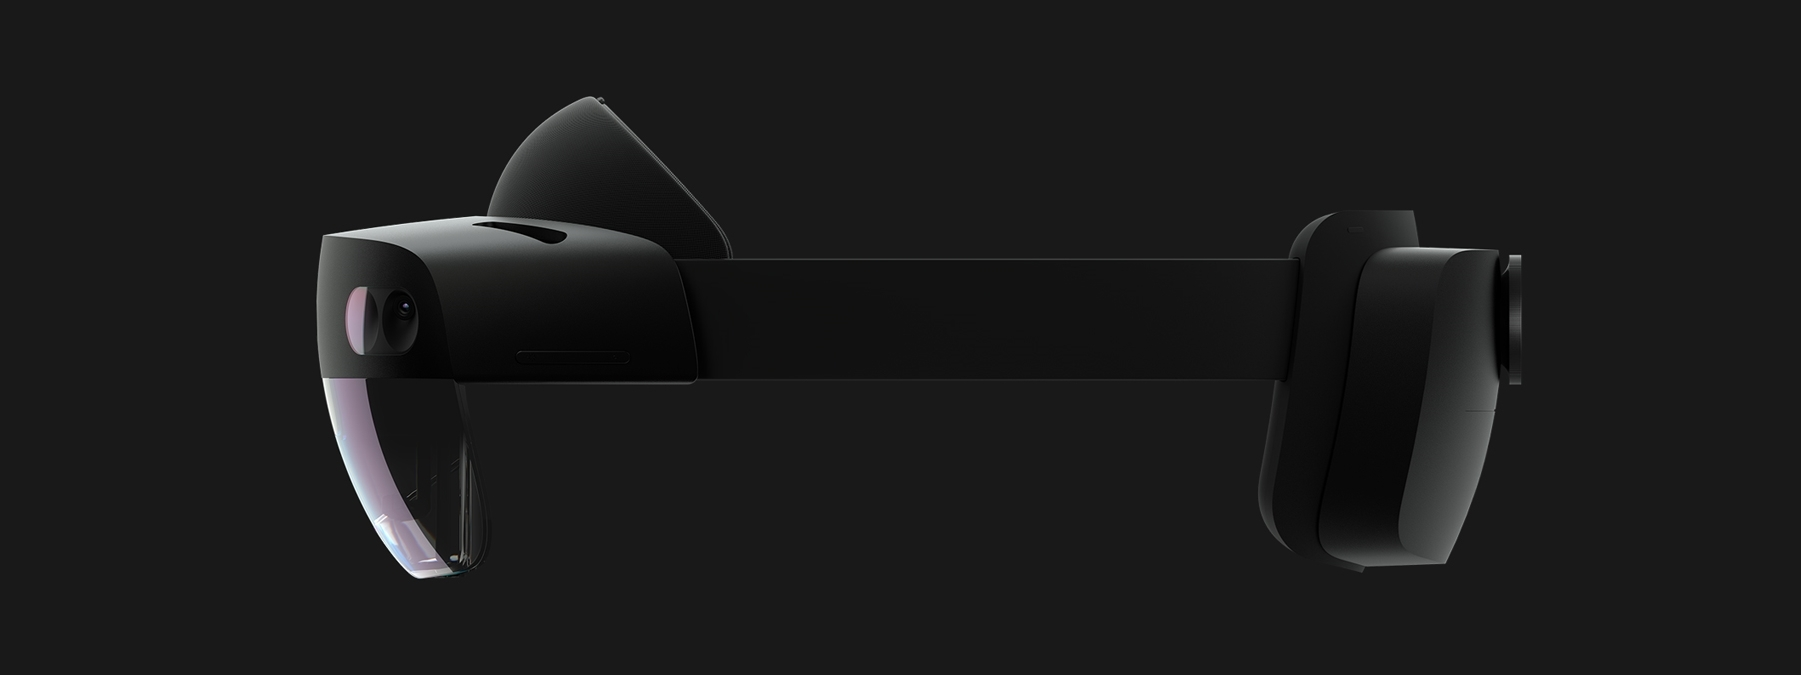
\includegraphics[width=0.9\linewidth]{figures/hololens.jpg}
    \caption[Side view of the HoloLens 2]{Side view of the HoloLens 2. Directly taken from \cite{HololensOverview}.}
      \label{fig:hololens}
\end{figure}

The HoloLens 2 (see fig. \ref{fig:hololens}) is a mixed reality headset developed by Microsoft and launched in 2019. It's the successor to the original HoloLens which was launched in 2016. Among the improvements are a larger field-of-view, fully articulated hand tracking, eye gaze tracking and a custom deep neural network core \cite{ResearchMode}. The HoloLens 2 runs Windows~10 and developers can create mixed reality apps by placing holograms in 3D space. See-through holographic lenses allow for an immersive mixed reality experience \cite{HololensHardware}.

\subsection{Hardware} \label{sec:holHardware}

The HoloLens 2 is designed to enable the creation of immersive mixed reality applications. It therefore is equipped with a lot of different sensors \cite{ResearchMode, HololensHardware}, some of them are:

\begin{itemize}
    \item RGB camera: Runs at up to 30fps with a resolution of up to 1080p. Able to take 8-MP photos.
    \item Depth camera: Is able to operate in two modes: Long Throw, which is a low-framerate ($\leq5$fps), far-depth mode and AHAT (Articulated HAnd Tracking) which is a high-framerate (45fps), near-depth mode.
    \item Four visible-light tracking (VLC) cameras: Placed at the left and right side of the headset and used for head tracking. Have a very wide field-of-view and produce greyscale images.
    \item Inertial Measurement Unit (IMU): Consists of an accelerometer, a gyroscope and a magnetometer. The accelerometer measures the linear acceleration, the gyroscope the rotation and the magnetometer the absolute orientation of the headset.
\end{itemize}

The placement of these sensors can be seen in fig. \ref{fig:holHardware}.

\begin{figure}
    \centering
    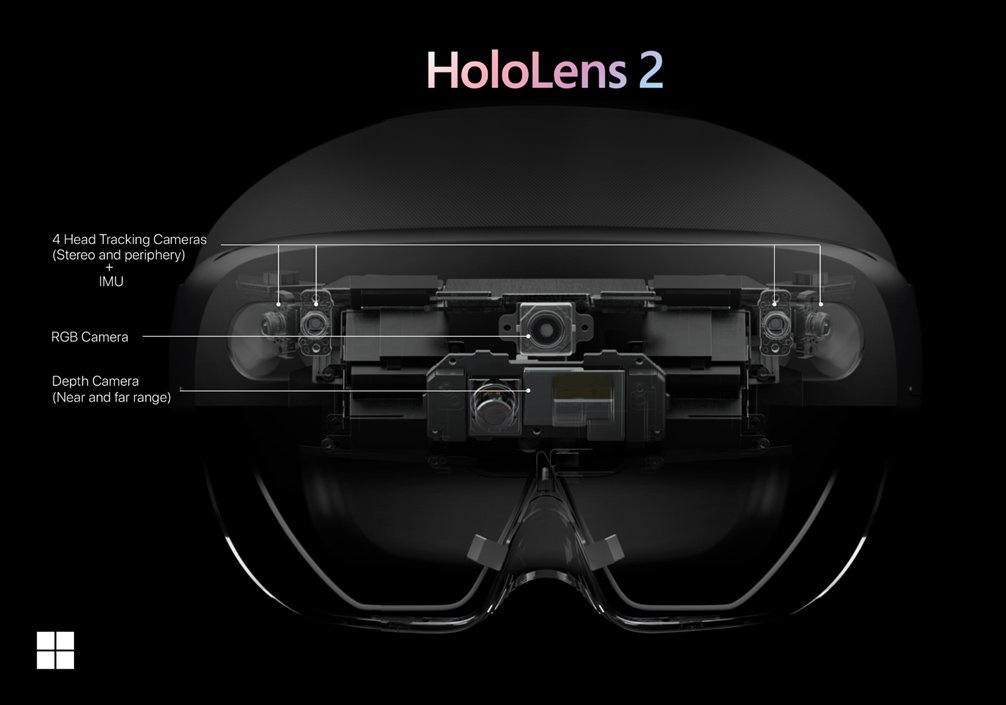
\includegraphics[width=0.9\linewidth]{figures/hololens2-front-view.png}
    \caption[Hololens 2 Hardware]{Image depicting the HoloLens 2 and some of its sensors, directly taken from Microsoft Docs \cite{HololensHardware}.}
      \label{fig:holHardware}
\end{figure}

The headset uses its various sensors to provide articulated hand tracking, eye gaze tracking, head tracking as well as spatial mapping out of the box. These tasks are performed by a special holographic processing unit with a deep neural network core which runs all native computer vision algorithms of the device. An additional Qualcomm Snapdragon 850 CPU is provided to run third-party applications. 

\subsection{Research Mode} \label{sec:ResearchMode}

The Windows Mixed Reality APIs \cite{DocMixedReality} provide access to a lot of functionality of the HoloLens 2 such as the capturing of camera frames and tracking of the the current head pose. However, these APIs don't allow for the developer to access the raw data streams of most sensors but only to the results of the processing of said streams for example the current head pose which is calculated using ineratial measurements. To address this, Microsoft introduced the Research Mode for HoloLens 2 \cite{ResearchMode} with the goal of encouraging contributions in the field of mixed reality by industrial and academic researchers. Research Mode needs to be specifically enabled in the Device Portal of the HoloLens 2 \cite{DevicePortal} and is not meant for applications targeted at end-users since they won't be able to run it. When enabled, Research Mode provides a set of \Cpp APIs to access various sensor streams of the HoloLens 2. Sensors exposed by Research Mode are the following:

\begin{itemize}
    \item VLC camera sensor: Provides access to the greyscale images produced by these cameras. Each camera can be targeted individually.
    \item Depth camera sensor: Provides access to the computed depth data for both modes described in sec. \ref{sec:holHardware} individually while also providing the raw infrared stream used to compute the depth map for both modes.
    \item IMU sensors: Provides access to measurement samples for each indiviual sensor. The API provides batches of measurement samples at a frequency between 12Hz and 22Hz.
\end{itemize}

Camera sensors and IMU sensors expose different functions. For example IMU sensors expose functions to either retrieve a single measurement sample per frame or a batch of measurement samples while camera sensors expose functions to map points from the three-dimensional camera space into the two-dimensional image space.

The API also provides extrinsic transformation matrices for each sensor relative to a static rigid node on the headset which represents the device origin and corresponds to the left front VLC camera. Each sensor returns a 4x4 transformation matrix to the this rigid node. To locate the sensors relative to other coordinate systems Research Mode allows for the retrieval of the GUID of the rigid node which can then be located relative to different coordinate systems using the HoloLens Perception API \cite{HololensPerception}. 

The authors of the Research Mode paper also provided a Github repository \cite{GithubRepoHololens2ForCV} which contains the full documentation for Research Mode as well as different example programs showcasing the use of Research Mode and code samples which can be used to develop with Research Mode.

\subsection{Development}

There are multiple options to develop mixed reality applications for HoloLens 2 \cite{DevMixedReality}. The most convenient ways are using one of the game engines Unity~\cite{Unity} or Unreal~\cite{Unreal}. Unity is especially well supported and runs the Mixed Reality Toolkit (MRTK) \cite{UnityMRTK} which is an open-source, cross-platform development kit for developing mixed reality applications. However there are multiple problems, when developing with Unity.

For one, Unity runs on C\# code while the used preexisting code for object tracking (see sec. \ref{sec:objectTracker}) is written in \Cpp. While it is possible to run DLLs (dynamic link libraries) compiled from \Cpp in Unity, the HoloLens 2 needs those DLLs to be compiled for UWP (Universal Windows Platform) and the ARM64 CPU architecture. Unity can run neither of those things in its built-in editor. Therefore we would need to compile those DLLs for different configurations, however the MRTK also does not support Research Mode at the current moment in time and Unity therefore is unable to create a correct build which we can then run on the HoloLens 2 without any modifications necessary. We can also not run any Research Mode code in the Unity editor. Couple this with long build times and the advantages of Unity for easily developing three-dimensional applications with nice user interfaces are outweighed by its disadvantages when working with \Cpp code and Research Mode.

Because of this, I decided to use Native OpenXR development for this application. It requires to handle the positioning and drawing of three-dimensional objects by oneself through the access of low level Mixed Reality Windows APIs but it is able to do this in pure \Cpp code. To make life a little easier I used the Cannon library for mixed reality development provided in \cite{GithubRepoHololens2ForCV} which uses DirectX and provides helper functions for perception and rendering.

\section{Object Tracker} \label{sec:objectTracker}

Robots have been used on assembly lines for a long time to great effect. They are usually cheaper, faster and more precise than human workers and don't need any breaks. However, these systems normally work in very constrained environments and cannot be used in more challenging scenarios like outside construction sites. 

The first challenge for such tasks is the tracking of objects in various environments. Early works used image gradients to detect edges and match them to objects \cite{GradientObjectTracking} and were then improved to allow for real-time object tracking \cite{RealTimeObjectTracking}. There is also work which improves tracking performance further, for example by online-learning object specific detectors \cite{OnlineLearningDetectors} or by incorporating color features \cite{ColorObjectTracking}.

Visual-inertial object tracking denotes object tracking with the addition of inertial measurements to improve tracking in cases where the sensor-head can be moving fast. For example in \cite{VisualInertialObjectTracking} the authors use inertial data to tune the parameters of feature detectors while also using camera images to calibrate the IMU to prevent drift (accumulated error over time).

This thesis uses the work of \cite{ViObjectTracker} which provides a system to track a sensor-head relative to multiple objects in real-time. It uses a probabilistic moving horizon estimator to fuse IMU measurements and camera frames to generate accurate pose estimates. The presented framework also provides functionalities for scene rendering and automatic tracking recovery and was showcased by accurately constructing a complex brick structure by hand as can be seen in fig. \ref{fig:objectTrackerExample}.

\begin{figure}
    \centering
    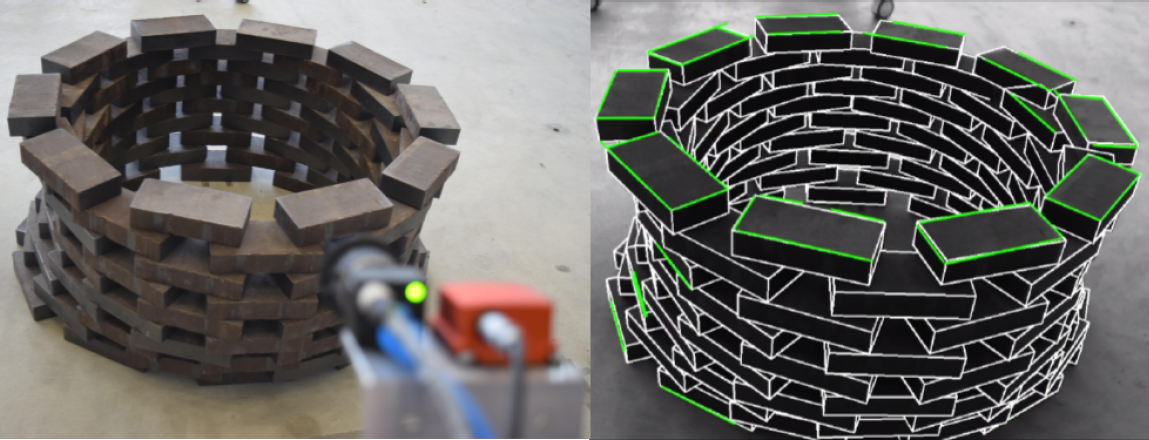
\includegraphics[width=0.9\linewidth]{figures/object_tracker_example.png}
    \caption[Object Tracker Brick Tower Showcase]{A brick tower built with the help of a visual-inertial tracking system. The left image shows the brick tower and the sensor-head while the right image shows the camera image overlaid with the rendered geometry. Directly taken from \cite{ViObjectTracker}.}
      \label{fig:objectTrackerExample}
\end{figure}

This work has since been further developed and currently consists of platform-independent \Cpp code and an application for Android phones. For the rest of this thesis we will refer to this code simply as the Object Tracker. The sensor fusion library used has since been open-sourced \cite{ConFusion} and the code further uses the ceres-solver~\cite{ceres-solver}, Eigen~\cite{eigen}, OpenCV~\cite{opencv_library} and Boost~\cite{boost} libraries.